\documentclass[border=2pt]{standalone}
\usepackage{tikz}
\begin{document}
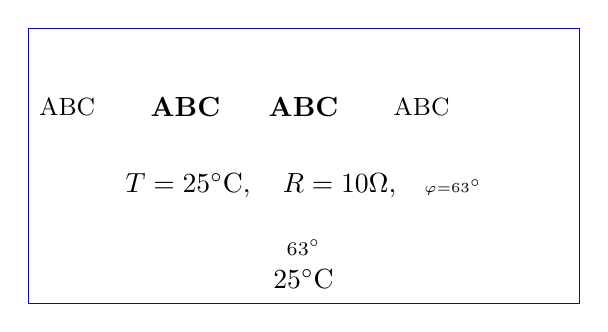
\begin{tikzpicture}[font=\small]
  \draw[blue,line width=.2pt] (-.5,-1.5) rectangle (6.5,2);
  \node at (0,1) {ABC};
  \node[font=\bfseries] at (1.5,1) {ABC};
  \begin{scope}[font=\bfseries]
    \node at (3,1) {ABC};
  \end{scope}
  \node at (4.5,1) {ABC};
  \node[font=\normalsize] at (3,0) {$T=25^\circ\mathrm{C},\quad R=10\Omega,\quad\scriptscriptstyle\varphi=63^\circ$};
  \node[font=\normalsize,align=center] at (3,-1) {$\scriptstyle 63^\circ$\\$25^\circ\mathrm{C}$};
\end{tikzpicture}
\end{document}
